% Options for packages loaded elsewhere
% Options for packages loaded elsewhere
\PassOptionsToPackage{unicode}{hyperref}
\PassOptionsToPackage{hyphens}{url}
\PassOptionsToPackage{dvipsnames,svgnames,x11names}{xcolor}
%
\documentclass[
  english,
  10pt,
  letterpaper,
  DIV=11,
  numbers=noendperiod]{scrartcl}
\usepackage{xcolor}
\usepackage[margin=1in]{geometry}
\usepackage{amsmath,amssymb}
\setcounter{secnumdepth}{5}
\usepackage{iftex}
\ifPDFTeX
  \usepackage[T1]{fontenc}
  \usepackage[utf8]{inputenc}
  \usepackage{textcomp} % provide euro and other symbols
\else % if luatex or xetex
  \usepackage{unicode-math} % this also loads fontspec
  \defaultfontfeatures{Scale=MatchLowercase}
  \defaultfontfeatures[\rmfamily]{Ligatures=TeX,Scale=1}
\fi
\usepackage{lmodern}
\ifPDFTeX\else
  % xetex/luatex font selection
\fi
% Use upquote if available, for straight quotes in verbatim environments
\IfFileExists{upquote.sty}{\usepackage{upquote}}{}
\IfFileExists{microtype.sty}{% use microtype if available
  \usepackage[]{microtype}
  \UseMicrotypeSet[protrusion]{basicmath} % disable protrusion for tt fonts
}{}
\makeatletter
\@ifundefined{KOMAClassName}{% if non-KOMA class
  \IfFileExists{parskip.sty}{%
    \usepackage{parskip}
  }{% else
    \setlength{\parindent}{0pt}
    \setlength{\parskip}{6pt plus 2pt minus 1pt}}
}{% if KOMA class
  \KOMAoptions{parskip=half}}
\makeatother
% Make \paragraph and \subparagraph free-standing
\makeatletter
\ifx\paragraph\undefined\else
  \let\oldparagraph\paragraph
  \renewcommand{\paragraph}{
    \@ifstar
      \xxxParagraphStar
      \xxxParagraphNoStar
  }
  \newcommand{\xxxParagraphStar}[1]{\oldparagraph*{#1}\mbox{}}
  \newcommand{\xxxParagraphNoStar}[1]{\oldparagraph{#1}\mbox{}}
\fi
\ifx\subparagraph\undefined\else
  \let\oldsubparagraph\subparagraph
  \renewcommand{\subparagraph}{
    \@ifstar
      \xxxSubParagraphStar
      \xxxSubParagraphNoStar
  }
  \newcommand{\xxxSubParagraphStar}[1]{\oldsubparagraph*{#1}\mbox{}}
  \newcommand{\xxxSubParagraphNoStar}[1]{\oldsubparagraph{#1}\mbox{}}
\fi
\makeatother


\usepackage{longtable,booktabs,array}
\newcounter{none} % for unnumbered tables
\usepackage{calc} % for calculating minipage widths
% Correct order of tables after \paragraph or \subparagraph
\usepackage{etoolbox}
\makeatletter
\patchcmd\longtable{\par}{\if@noskipsec\mbox{}\fi\par}{}{}
\makeatother
% Allow footnotes in longtable head/foot
\IfFileExists{footnotehyper.sty}{\usepackage{footnotehyper}}{\usepackage{footnote}}
\makesavenoteenv{longtable}
\usepackage{graphicx}
\makeatletter
\newsavebox\pandoc@box
\newcommand*\pandocbounded[1]{% scales image to fit in text height/width
  \sbox\pandoc@box{#1}%
  \Gscale@div\@tempa{\textheight}{\dimexpr\ht\pandoc@box+\dp\pandoc@box\relax}%
  \Gscale@div\@tempb{\linewidth}{\wd\pandoc@box}%
  \ifdim\@tempb\p@<\@tempa\p@\let\@tempa\@tempb\fi% select the smaller of both
  \ifdim\@tempa\p@<\p@\scalebox{\@tempa}{\usebox\pandoc@box}%
  \else\usebox{\pandoc@box}%
  \fi%
}
% Set default figure placement to htbp
\def\fps@figure{htbp}
\makeatother


% definitions for citeproc citations
\NewDocumentCommand\citeproctext{}{}
\NewDocumentCommand\citeproc{mm}{%
  \begingroup\def\citeproctext{#2}\cite{#1}\endgroup}
\makeatletter
 % allow citations to break across lines
 \let\@cite@ofmt\@firstofone
 % avoid brackets around text for \cite:
 \def\@biblabel#1{}
 \def\@cite#1#2{{#1\if@tempswa , #2\fi}}
\makeatother
\newlength{\cslhangindent}
\setlength{\cslhangindent}{1.5em}
\newlength{\csllabelwidth}
\setlength{\csllabelwidth}{3em}
\newenvironment{CSLReferences}[2] % #1 hanging-indent, #2 entry-spacing
 {\begin{list}{}{%
  \setlength{\itemindent}{0pt}
  \setlength{\leftmargin}{0pt}
  \setlength{\parsep}{0pt}
  % turn on hanging indent if param 1 is 1
  \ifodd #1
   \setlength{\leftmargin}{\cslhangindent}
   \setlength{\itemindent}{-1\cslhangindent}
  \fi
  % set entry spacing
  \setlength{\itemsep}{#2\baselineskip}}}
 {\end{list}}
\usepackage{calc}
\newcommand{\CSLBlock}[1]{\hfill\break\parbox[t]{\linewidth}{\strut\ignorespaces#1\strut}}
\newcommand{\CSLLeftMargin}[1]{\parbox[t]{\csllabelwidth}{\strut#1\strut}}
\newcommand{\CSLRightInline}[1]{\parbox[t]{\linewidth - \csllabelwidth}{\strut#1\strut}}
\newcommand{\CSLIndent}[1]{\hspace{\cslhangindent}#1}

\ifLuaTeX
\usepackage[bidi=basic,shorthands=off]{babel}
\else
\usepackage[bidi=default,shorthands=off]{babel}
\fi
\ifLuaTeX
  \usepackage{selnolig} % disable illegal ligatures
\fi


\setlength{\emergencystretch}{3em} % prevent overfull lines

\providecommand{\tightlist}{%
  \setlength{\itemsep}{0pt}\setlength{\parskip}{0pt}}



 


\KOMAoption{captions}{tableheading}
\makeatletter
\@ifpackageloaded{caption}{}{\usepackage{caption}}
\AtBeginDocument{%
\ifdefined\contentsname
  \renewcommand*\contentsname{Table of contents}
\else
  \newcommand\contentsname{Table of contents}
\fi
\ifdefined\listfigurename
  \renewcommand*\listfigurename{List of Figures}
\else
  \newcommand\listfigurename{List of Figures}
\fi
\ifdefined\listtablename
  \renewcommand*\listtablename{List of Tables}
\else
  \newcommand\listtablename{List of Tables}
\fi
\ifdefined\figurename
  \renewcommand*\figurename{Figure}
\else
  \newcommand\figurename{Figure}
\fi
\ifdefined\tablename
  \renewcommand*\tablename{Table}
\else
  \newcommand\tablename{Table}
\fi
}
\@ifpackageloaded{float}{}{\usepackage{float}}
\floatstyle{ruled}
\@ifundefined{c@chapter}{\newfloat{codelisting}{h}{lop}}{\newfloat{codelisting}{h}{lop}[chapter]}
\floatname{codelisting}{Listing}
\newcommand*\listoflistings{\listof{codelisting}{List of Listings}}
\makeatother
\makeatletter
\makeatother
\makeatletter
\@ifpackageloaded{caption}{}{\usepackage{caption}}
\@ifpackageloaded{subcaption}{}{\usepackage{subcaption}}
\makeatother
\usepackage{bookmark}
\IfFileExists{xurl.sty}{\usepackage{xurl}}{} % add URL line breaks if available
\urlstyle{same}
% fallback for those not using the hyperref driver hyperxmp:
\makeatletter
\@ifundefined{xmpquote}{\newcommand{\xmpquote}[1]{#1}}{}
\makeatother
\hypersetup{
  pdftitle={Phase-Gram},
  pdfauthor={Complex--Itô Random-Walk Research Project},
  pdflang={en},
  pdfkeywords={\xmpquote{correlation matrix}, \xmpquote{angles
parameterization}, \xmpquote{Gram matrices}, \xmpquote{stochastic
correlation}, \xmpquote{Gauss-Hermite quadrature}},
  colorlinks=true,
  linkcolor={blue},
  filecolor={Maroon},
  citecolor={Blue},
  urlcolor={Blue},
  pdfcreator={LaTeX via pandoc}}


\title{Phase-Gram}
\usepackage{etoolbox}
\makeatletter
\providecommand{\subtitle}[1]{% add subtitle to \maketitle
  \apptocmd{\@title}{\par {\large #1 \par}}{}{}
}
\makeatother
\subtitle{Correlation-Matrix Processes with Exact Finite-Time Law from
Gaussian-Driven Triangular Angles}
\author{Complex--Itô Random-Walk Research Project}
\date{August 21, 2026}
\begin{document}
\maketitle
\begin{abstract}
We turn the canonical triangular-angle (Gram) parameterization of
correlation matrices --- a static calibration tool in the LIBOR-market-
model literature (Rebonato--Jäckel; Rapisarda--Brigo--Mercurio) --- into
a stochastic process by driving each angle with an independent Brownian
motion. Three structural payoffs follow. First, the matrix
\(R_t=B(\theta_t)B(\theta_t)^\top\) is positive semidefinite with unit
diagonal \emph{by construction}: no repulsion parameters, no boundary
conditions, in contrast with Jacobi-type matrix diffusions. Second, the
angle vector is jointly Gaussian, so the finite-time law of the entire
matrix is exact: every European functional \(E[h(R_T)]\) reduces to a
\(d=n(n-1)/2\)-dimensional Gauss--Hermite product integral; pairwise
marginals are closed form (\(\cos\) of a Gaussian). Third, induced entry
drifts are explicit --- for the free three-asset entry,
\(\mu_{R_{23}}=-\tfrac12(\sigma_\alpha^2+\sigma_\beta^2)R_{23}
-\tfrac12\sigma_\gamma^2\sin\alpha\sin\beta\cos\gamma\) --- so entries
mean-revert endogenously through Itô curvature, without any reversion
parameter. We verify PSD at machine zero over random angle draws, closed
marginals and Gauss--Hermite prices against bridge-corrected Monte Carlo
within \textasciitilde1--3 standard errors, and analytic drifts to third
decimals. European correlation-matrix derivatives --- digitals and calls
on entries, average-correlation payoffs --- become deterministic
quadratures where the audited literature uses simulation.
\end{abstract}

\renewcommand*\contentsname{Table of contents}
{
\setcounter{tocdepth}{2}
\tableofcontents
}

\textbf{Mathematics Subject Classification (2020):} 60H10, 60J60, 91G20,
65D32.

\textbf{JEL classification:} G13, C63.

\section{Introduction}\label{sec-introduction}

A correlation matrix must live on the compact set of symmetric positive-
semidefinite matrices with unit diagonal. The two audited strategies for
building \emph{processes} there pull in opposite directions. Jacobi-type
diffusions respect an SDE but need parameter restrictions to keep the
boundary unreachable and yield no closed-form entry laws. Angle
parameterizations --- Rebonato--Jäckel's spherical rows (Rebonato and
Jäckel 1999) and the canonical triangular refinement of Rapisarda et al.
(2002) --- guarantee admissibility by construction but were conceived as
\emph{static} calibration tools.

The Phase-Gram construction takes the second route dynamic: drive every
canonical angle by its own Brownian motion. Admissibility survives
tautologically, and --- the new content --- \textbf{exactness} arrives
free: Gaussian angles make the whole matrix exactly
finitely-dimensional-law'd.

\section{Construction}\label{sec-construction}

\subsection{Triangular angles}\label{triangular-angles}

For \(n\) assets, let \(d=n(n-1)/2\) angles \(\theta_{i,j}\), \(i>j\).
Rows of the Cholesky factor \(B\) are spherical coordinates:

\[
b_{i,k}=\cos\theta_{i,k}\prod_{m<k}\sin\theta_{i,m},\qquad
b_{i,i}=\prod_{m<i}\sin\theta_{i,m},
\]

and \(R=B B^\top\). For \(n=3\): \(x_1=e_1\),
\(x_2=(\cos\alpha,\sin\alpha,0)\),
\(x_3=(\cos\beta,\sin\beta\cos\gamma,\sin\beta\sin\gamma)\), so

\[
R_{23}=\cos\alpha\cos\beta+\sin\alpha\sin\beta\cos\gamma .
\]

\subsection{Dynamics}\label{dynamics}

\[
d\theta_{ij}=\sigma_{ij}\,dW_{ij},\qquad \text{independent across pairs.}
\]

\textbf{Proposition (admissibility).} \emph{\(R_t\) is symmetric, PSD,
and unit- diagonal for every angle configuration and every \(t\);
minimum eigenvalues over 2,000 random draws are at machine zero.}

\textbf{Theorem (exact finite-time law).} \emph{\(\theta_T\) is jointly
Gaussian with independent coordinates, hence for any measurable \(h\),}
\[E[h(R_T)] = \int h(R(\theta))\,\bigotimes_{k=1}^{d}\varphi(d\theta_k),\]
\emph{a product Gauss--Hermite rule in \(d\) dimensions. Pairwise
marginals are closed form:} \(R_{12}(T)=\cos\Theta\) \emph{with}
\(\Theta\sim N(\theta_0,\sigma^2T)\)\emph{, so}
\(E[R_{12}(T)]=e^{-\sigma^2T/2}\cos\theta_0\) \emph{and}
\(E[R_{12}^2]=\tfrac12(1+e^{-2\sigma^2T}\cos2\theta_0)\).

\subsection{Induced entry dynamics}\label{induced-entry-dynamics}

Itô's lemma gives explicit drifts; for the free three-asset entry,

\[
\mu_{R_{23}}=-\tfrac12(\sigma_\alpha^2+\sigma_\beta^2)\,R_{23}
-\tfrac12\sigma_\gamma^2\sin\alpha\sin\beta\cos\gamma :
\]

entries mean-revert through curvature \textbf{without any reversion
parameter} --- the trigonometric boundedness does the work that Jacobi
repulsion parameters do elsewhere.

\section{Verification}\label{sec-verification}

{\def\LTcaptype{none} % do not increment counter
\begin{longtable}[]{@{}
  >{\raggedright\arraybackslash}p{(\linewidth - 2\tabcolsep) * \real{0.5000}}
  >{\raggedright\arraybackslash}p{(\linewidth - 2\tabcolsep) * \real{0.5000}}@{}}
\toprule\noalign{}
\begin{minipage}[b]{\linewidth}\raggedright
check
\end{minipage} & \begin{minipage}[b]{\linewidth}\raggedright
result
\end{minipage} \\
\midrule\noalign{}
\endhead
\bottomrule\noalign{}
\endlastfoot
PSD / unit diagonal / symmetry & machine zero / 1e-12 / exact \\
deterministic limit equals static RBM map & exact \\
\(R_{23}\) entry identity vs general map & \(10^{-12}\) \\
\(E[R_{12}]\), sd: closed form vs MC (300k) & within 1 SE \\
\(E[R_{23}]\), sd: GH(30/dim) vs MC & within \textasciitilde1 SE \\
short-horizon drift, three states, 400k paths each & analytic vs
empirical ≤3rd decimal \\
\end{longtable}
}

Analytic-vs-MC drift comparison:

{\def\LTcaptype{none} % do not increment counter
\begin{longtable}[]{@{}lll@{}}
\toprule\noalign{}
start \((\alpha,\beta,\gamma)\) & empirical & analytic \\
\midrule\noalign{}
\endhead
\bottomrule\noalign{}
\endlastfoot
(0.3, −0.2, 0.5) & −0.4316 & −0.4298 \\
(1.0, 0.8, −0.6) & −0.5589 & −0.5594 \\
(−0.9, 0.4, 1.2) & −0.2212 & −0.2039 \\
\end{longtable}
}

\section{Correlation-matrix derivatives}\label{sec-derivatives}

European payoffs on entries price as deterministic product quadratures
((\textbf{tab-calls?})):

{\def\LTcaptype{none} % do not increment counter
\begin{longtable}[]{@{}lll@{}}
\toprule\noalign{}
strike \(K\) & call on \(R_{23}(T)\): GH & MC (SE) \\
\midrule\noalign{}
\endhead
\bottomrule\noalign{}
\endlastfoot
−0.2 & 0.77088 & 0.77159 (0.00070) \\
0.0 & 0.59329 & 0.59381 (0.00063) \\
+0.2 & 0.42673 & 0.42727 (0.00053) \\
+0.4 & 0.27566 & 0.27601 (0.00041) \\
+0.6 & 0.14564 & 0.14598 (0.00028) \\
\end{longtable}
}

Digital \(R_{23}(T)\ge0.4\): 0.71248 vs MC 0.70950. Kinked payoffs
converge polynomially (20→40 nodes differ by 2.4e-4). The exact term
structure of \(E[R_{23}(t)]\) follows from the same machinery
(Figure~\ref{fig-term}).

\begin{figure}[tbp]

\centering{

\pandocbounded{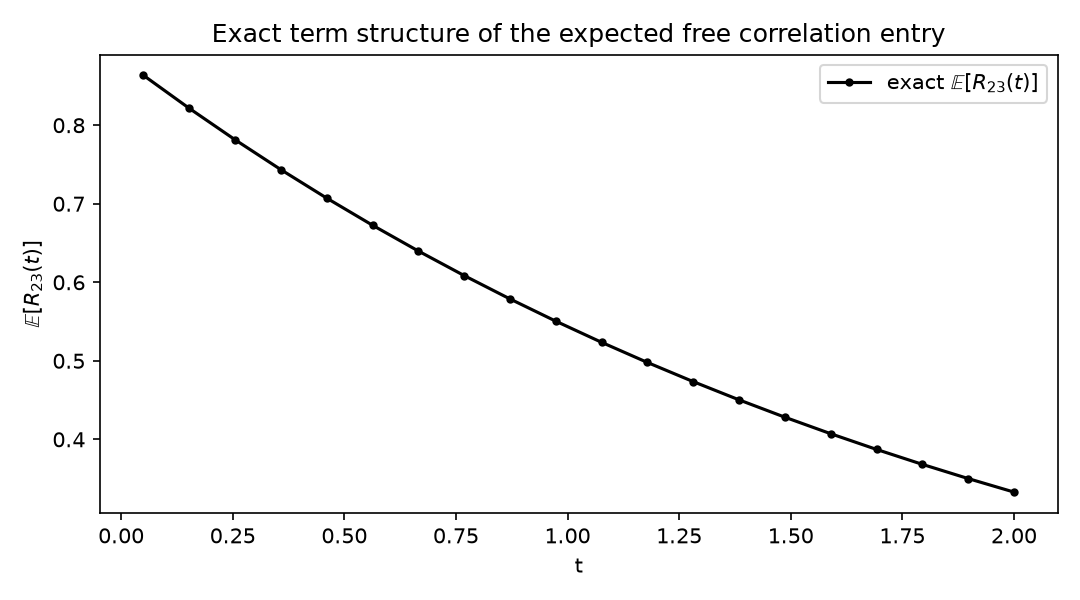
\includegraphics[keepaspectratio]{figures/phase10_term_structure.png}}

}

\caption{\label{fig-term}Exact term structure of the expected free
correlation entry.}

\end{figure}%

\section{Related literature}\label{sec-related}

Rebonato and Jäckel (1999) introduced the angles for rank reduction and
noted their unconditional admissibility; Rapisarda et al. (2002)
canonicalized them (``triangular angles'', one-to-one with \(M(M-1)/2\)
parameters) for static calibration in the LIBOR market model.
Brigo--Mercurio's ``the basis goes stochastic'' makes basis volatilities
stochastic but prices by simulation. Jacobi matrix diffusions (Ahdida
and Alfonsi 2013) admit exact schemes but not entry laws. None of the
audited sources drives the canonical angles with independent Gaussians,
and none claims exact finite-time laws or deterministic
correlation-derivative pricing.

\section{Limitations}\label{sec-limitations}

Product-rule Gauss--Hermite costs \(O(n_{\text{pts}}^d)\): comfortable
to \(d=4\)--5 assets; beyond that, sparse grids or the Monte Carlo
benchmark route take over. Angle volatilities are free parameters ---
calibrating them to quoted correlation derivatives is now a likelihood
problem on closed-form prices, which we flag as the natural
continuation. The Gaussian driver has no stationary law; long horizons
are diffusive by design.

\section{Conclusion}\label{sec-conclusion}

One line of dynamics --- independent Brownian angles --- converts a
static parameterization into the first correlation-matrix process whose
entire European law is a quadrature. Constraint-free admissibility,
closed-form marginals, analytic drifts, and deterministic pricing arrive
together.

\section{Reproducibility}\label{sec-repro}

Environment: conda \texttt{phase3-paper} (Python 3.12.13, numpy 2.5.1,
scipy 1.18.0). Notebook \texttt{notebooks/phase10\_matrix.ipynb}
(\textasciitilde8 s, seed 20260821); module \texttt{phase10\_matrix.py};
tests \texttt{tests/test\_phase10\_matrix.py} (11/11).

\protect\phantomsection\label{refs}
\begin{CSLReferences}{1}{1}
\bibitem[\citeproctext]{ref-ahdida2013}
Ahdida, Aurélien, and Aurélien Alfonsi. 2013. {``Exact Mean-Rate Laplace
Transforms and Exact Simulation of Jacobi-Type Processes.''}
\emph{Annals of Applied Probability} 23 (6): 2360--94.

\bibitem[\citeproctext]{ref-rbm2002}
Rapisarda, Francesco, Damiano Brigo, and Fabio Mercurio. 2002.
{``Parameterizing Correlations: A Geometric Interpretation.''}
\emph{Preprint, Banca IMI}.

\bibitem[\citeproctext]{ref-rebonato1999}
Rebonato, Riccardo, and Peter Jäckel. 1999. \emph{The Most General
Methodology to Create a Valid Correlation Matrix for Risk Management and
Option Pricing Purposes}.

\end{CSLReferences}




\end{document}
